

\chapter{Graphs, Networks, and Clustering}
\label{c:graphs}


A crucial part of data science consists of the study of networks. Network science, or graph theory, unifies the study of diverse types of networks, such as social networks, protein-protein interaction networks, gene-regulation networks, and the internet. In this chapter we introduce graph theory and treat the problem of clustering, to identify similar data points, or vertices, in (network) data.

\section{PageRank}

Before we introduce the formalism of graph theory, we describe the celebrated PageRank algorithm. This algorithm is a principal component\footnote{It is difficult to resist using this pun.} behind web search algorithms, in particular in Google. The goal of PageRank is to quantitatively rate the importance of each page on the web, allowing the search algorithm to rank the pages and thereby present to the user the more important pages first.
Search engines such as Google have to carry out three basic steps:\footnote{Another important component of modern search engines is personalization, which we do not discuss here.}
\begin{itemize}
\setlength{\parsep}{-0.3ex}
\setlength{\itemsep}{-0.3ex}
\item Crawl the web and locate all, or as many as possible, accessible webpages.
\item Index the data of the webpages from step 1, so that they can be searched efficiently for relevant
key words or phrases.
\item Rate the importance of each page in the database, so that when a user does
a search and the subset of pages in the database with the desired information
has been found, the more important pages can be presented first.
\end{itemize}
Here, we will focus on the third step. We follow mainly the derivation in~\cite{Bryan2006}. We aim to develop a score of importance for each webpage. A score will be a
non-negative number. A key idea in assigning a score to any given webpage is that the page's score is derived from the
links made to that page from other webpages --- ``A person is important not if it knows a lot of people, but if a lot of
people know that person''. 

Suppose the web of interest contains $n$ pages, each page indexed by an integer $k$,
$1 \le k \le n$. A typical example is illustrated in Figure~\ref{fig:web}, in which an arrow from page
$k$ to page $j$ indicates a link from page $k$ to page $j$. Such a web is an example of a
directed graph. The links to a given page are called
the backlinks for that page.
We will use $x_k$ to denote the importance score of page $k$ in the web. $x_k$
is nonnegative and $x_j > x_k$ indicates that page $j$ is more important than page $k$.

\begin{figure}[h]
\begin{center}

\includegraphics[width=40mm]{figures/Chapter4-web}
\end{center}
\caption{A toy example of the Internet}
\label{fig:web}
\end{figure}

A very simple approach is to take $x_k$ as the number of backlinks for page $k$. In
the example in Figure~\ref{fig:web}, we have $x_1 = 2, x_2 = 1, x_3 = 3$, and $x_4 = 2$, so that page 3
is the most important, pages 1 and 4 tie for second, and page 2 is least important. A
link to page $k$ becomes a vote for page $k$'s importance.
This approach ignores an important feature one would expect a ranking algorithm
to have, namely, that a link to page $k$ from an important page should boost page $k$'s
importance score more than a link from an unimportant page.
In the web of Figure~\ref{fig:web}, pages 1 and 4 both have two backlinks: each links to the other, but the second backlink from page
1 is from the seemingly important page 3, while the second
backlink for page 4 is from the relatively unimportant page 2. As such, perhaps the algorithm should rate
the importance of page 1 higher than that of page 4.

As a first attempt at incorporating this idea, let us compute the score of page $j$ as
the sum of the scores of all pages linking to page $j$. For example, consider the web
in our toy example. The score of page 1 would be determined by the relation $x_1 = x_3 + x_4$.
However, since $x_3$ and $x_4$ will depend on $x_1$, this seems like a circular definition, since it is
self-referential (it is exactly this self-referential property that will establish a connection to eigenvector
problems!).

We also seek a scheme in which a webpage does not gain extra influence
simply by linking to lots of other pages. We can do this by reducing the impact of each link, as more and more outgoing 
links are added to a webpage. If page $j$ contains $n_j$ links, one of which
links to page $k$, then we will boost page $k$'s score by $x_j/n_j$, rather than by $x_j$. In
this scheme, each webpage gets a total of one vote, weighted by that web page's score,
that is evenly divided up among all of its outgoing links. To quantify this for a web
of $n$ pages, let $L_k \subset \{1,2,\dots, n\}$ denote the set of pages with a link to page $k$, that
is, $L_k$ is the set of page $k$'s backlinks. For each $k$ we require
$$x_k = \sum_{j \in L_k} \frac{x_j}{n_j},$$
where $n_j$ is the number of outgoing links from page $j$. 

If we apply these scheme to the toy example in Figure~\ref{fig:web}, then for page 1 we have
$x_1 = x_3/1 + x_4/2$,  since pages 3 and 4 are backlinks for page 1 and page 3 contains
only one link, while page 4 contains two links (splitting its vote in half). Similarly,
$x_2 = x_1/3, x_3 = x_1/3 + x_2/2 + x_4/2$, and $x_4 = x_1/3 + x_2/2$. These conditions can be expressed as linear
system of equations $Ax =x$, where $x=[x_1,x_2,x_3,x_4]^T$ and 
$$A = 
\begin{bmatrix}
0 & 0 & 1 & \frac{1}{2} \\
\frac{1}{3} & 0 & 0 & 0 \\
\frac{1}{3} & \frac{1}{2} & 0 & \frac{1}{2} \\
\frac{1}{3} & \frac{1}{2} & 0 & 0 
\end{bmatrix}
$$
Thus, we end up with an eigenvalue/eigenvector problem: Find the eigenvector $x$ of the matrix $A$, associated with the
eigenvalue 1. We note that $A$ is a column-stochastic matrix, since it is a square matrix for which all of its
entries are nonnegative and the entries in each column sum to 1. If we build a random walk on the internet where each link is clicked with equal probability then $A_{ij}$ is the probability that a random walked in page $j$ goes to page $i$. Later, in Chapter~\ref{c:diffusion}, we will use random walks on (undirected) graphs in order to embed their nodes in euclidean space, we note that, in that context, we will mostly work with $M=A^T$ the matrix for which  $M_{ij}$ corresponds to the probability of taking step from $i$ to $j$. Stochastic matrices arise in the study of Markov chains and in a variety of modeling problems in economics and
operations research.  See e.g.~\cite{HJ90} for more details on stochastic matrices. The fact that 1 is an eigenvalue of $A$ is not just coincidence in this example, but holds true in general for stochastic matrices. 

\begin{proposition}\label{prop:columnstochastichaseig1}
A column-stochastic matrix $A$ has an eigenvalue equal to 1 and 1 is also its largest eigenvalue.
\end{proposition}

\begin{proof}
Let $A$ be an $n\times n$ column-stochastic matrix.
We first note that $A$ and $A^T$ have the same eigenvalues (their eigenvector will usually be different though).
Let $\mathbf{1} = [1,1,\dots,1]^T$ be the vector of length $n$ which has all ones as entries. Since $A$ is
column-stochastic, we have $A^T \mathbf{1} = \mathbf{1}$ (since all columns of $A$ sum up to 1). Hence $\mathbf{1}$ is an eigenvector of
$A^T$ (but not of $A$) with eigenvalue 1. Thus 1 is also an eigenvalue of $A$.

To show that 1 is the largest eigenvalue of $A$ we apply the Gershgorin Circle Theorem~\cite{HJ90} to $A^T$. Consider
row $k$ of $A^T$. Let us call the diagonal element $a_{k,k}$ and the radius will be
$\sum_{i \neq k} |a_{k,i}| = \sum_{i \neq k} a_{k,i}$ since $a_{k,i} \ge 0$. This is a circle with its center
at $a_{k,k} \in [0,1]$ and with radius $\sum_{i \neq k} a_{k,i} = 1 - a_{k,k}$. Hence, this circle has 1 on its
perimeter. This holds for all Gershgorin circles for this matrix.  Thus, since all eigenvalues lie in the
union of the Gershgorin circles, all eigenvalues $\lambda_i$ satisfy $|\lambda_i| \le 1$.

\end{proof}


In our example, we obtain as eigenvector $x$ of $A$ associated with eigenvalue 1 the vector
$x = [x_1,x_2,x_3,x_4]^T$ with entries
 $x_1 = \frac{12}{31}, x_2 = \frac{4}{31}, x_3 = \frac{9}{31}$, and $x_4 =
\frac{6}{31}$. Hence, perhaps somewhat surprisingly, page 3 is no longer the most important one, but page 1.
This can be explained by the fact, that the in principle quite important page 3 (which has three webpages linking to
it) has only one outgoing link, which gets all its ``voting power'', and that link points to page 1.


In reality, $A$ can easily be of size a billion times a billion. Fortunately, we do not need compute all eigenvectors
of $A$, only the eigenvector associated with the eigenvalue 1, which, as we know, is also the largest eigenvalue of $A$.
This in turn means we can resort to standard {\em power iteration} to compute $x$ fairly efficiently (and we can also make
use of the fact that $A$ will be a sparse matrix, i.e., many of its entries will be zero).
The actual PageRank algorithms adds some minor modifications,\footnote{One such modification is the addition of very small weight edges between every pair of pages, corresponding to a ``random teleport'' of the random walker (or web crawler) that happens with very low probability. One advantage this brings is that the networks becomes irreducible. A reducible directed graph is one for which there are nodes $u$ and $v$ for which there is no directed path from $u$ to $v$, if a networks is not reducible, it is called irreducible.} but the essential idea is as described above.


The idea to use eigenvectors for ranking dates back to the late 1800s to the work of Edmund Landau in the context
of ranking in chess tournaments, it was actually Landau's first mathematical paper when he was 18 years old~\cite{Landau1895Turnierresultate} (with a follow-up later~\cite{Landau1914Preisverteilung}). You
can read about this nice story in~\cite{sinn2022landau}.




\section{Graphs and clustering}

We now introduce the formalism for undirected\footnote{The previous Chapter featured directed graphs, in which edges (links) have a meaningful direction. In what follows we will focus in undirected graphs in which an edge represents a connection, without meaningful direction.} graphs, one of the main objects of study in what follows. A graph $G = (V,E)$ contains a set of nodes $V=\left\{v_1,\dots,v_n\right\}$ and edges $E\subseteq {V \choose 2 }$. An edge $(i,j)\in E$ if $v_i$ and $v_j$ are connected. Figure \ref{fig:Petersen} depicts one of the graph theorists' favorite examples, the Petersen graph\footnote{The Petersen graph is often used as a counter-example in graph theory.}.


\begin{figure}[h]
\begin{center}

\includegraphics[width=0.4\textwidth]{figures/Chapter4-PetersenGraph.png}
\caption{The Petersen graph}
\label{fig:Petersen}
\end{center}
 
\end{figure}



Let us recall some concepts about graphs that we will need.
\begin{itemize}
\item A graph is {\em connected} if, for all pairs of vertices, there is a path between these vertices in the graph. The number of connected components is simply the size of the smallest partition of the nodes into connected subgraphs. The Petersen graph is connected (and thus it has only $1$ connected component).

\item A {\em clique} of a graph $G$ is a subset $S$ of its nodes such that the subgraph corresponding to it is complete. In other words $S$ is a clique if all pairs of vertices in $S$ share an edge. The clique number $c(G)$ of $G$ is the size of the largest clique of $G$. The Petersen graph has a clique number of $2$.

\item An {\em independent set} of a graph $G$ is a subset $S$ of its nodes such that no two nodes in $S$ share an edge. Equivalently it is a clique of the complement graph $G^c \defeq \left(V,E^c\right)$. The independence number of $G$ is simply the clique number of $S^c$. The Petersen graph has an independence number of $4$.

\end{itemize}

A particularly useful way to represent a graph is through its adjacency matrix. Given a graph $G=(V,E)$ on $n$ nodes ($|V|=n$), we define its adjacency matrix $A \in \RR^{n\times n}$ as the symmetric matrix with entries
\begin{equation}
 \label{adjacencymatrix}   
A_{ij} = \left\{  \begin{array}{ll} 1 & \text{ if } (i,j)\in E, \\ 0 & \text{otherwise}.   \end{array}   \right.
\end{equation}


Sometimes, we will consider weighted graphs $G=(V,E,W)$, where edges may have weights $w_{ij}$ that are non-negative $w_{ij}\geq 0$ and symmetric $w_{ij} = w_{ji}$.

Much of the sequel will deal with graphs. Chapter~\ref{c:diffusion} will treat (network) data visualization, dimension reduction, and embeddings of graphs in Euclidean space. Chapter~\ref{c:community} will introduce and study important random graph models. The rest of this Chapter will be devoted to spectral graph theory, clustering, and graph metrics. 

Clustering is one of the central tasks in machine learning. Given a set of data points, or nodes of a graph, the purpose of clustering is to partition the data into a set of clusters where data points assigned to the same cluster correspond to similar data points (depending on the context, it could be for example having small distance to each other if the points are in Euclidean space, or having high connectivity if on a graph). We will start with an example of clustering points in Euclidean space, and later move back to graphs.

\begin{figure}[h]
\begin{center}

\includegraphics[width=0.8\textwidth]{figures/Chapter4-fig_3_clusters.pdf}
\caption{Example of points separated into clusters. By using different symbols and colors, the three clusters appear more distinct than they actually are. }
\label{figure:3:clustering_00}
\end{center}
\end{figure}

\section{$k$-means clustering}

One the most popular methods used for clustering is $k$-means clustering. Given $x_1,\dots,x_n\in\RR^p$ the $k$-means clustering partitions the data points into clusters $S_1\cup \dots \cup S_k$ with centers $\mu_1,\dots,\mu_k\in\RR^p$ as the solution to:
\begin{equation}\label{eq:3:kmeans_obj}
\min_{\text{partition}\ \substack{S_1,\dots,S_k \\ \mu_1,\dots,\mu_k}}\sum_{l=1}^k \sum_{i\in S_l} \left\|  x_i - \mu_l\right\|^2.
\end{equation}
Note that, given the partition, the optimal centers are given by
\[
\mu_l = \frac1{\left| S_l \right|} \sum_{i\in S_l}x_i.
\]

Lloyd's algorithm~\cite{Lloyd:kmeans} (also sometimes known as the $k$-means algorithm), is an iterative algorithm that alternates between
\begin{itemize}
\item Given centers $\mu_1,\dots,\mu_k$, assign each point $x_i$ to the cluster $S_l$ with nearest center 
\[
l=\argmin_{l=1,\dots, k}\left\|  x_i - \mu_l \right\|.
\]
\item Update the centers $\mu_l =  \frac1{\left| S_l \right|} \sum_{i\in S_l}x_i$.
\end{itemize}

Unfortunately, Lloyd's algorithm is not guaranteed to converge to the solution of~\eqref{eq:3:kmeans_obj}. Indeed, Lloyd's algorithm oftentimes gets stuck in local optima of~\eqref{eq:3:kmeans_obj}. In the following we will discuss convex relaxations for clustering, which can be used as an alternative algorithmic approach to Lloyd's algorithm, but since optimizing~\eqref{eq:3:kmeans_obj} is $NP$-hard there is no polynomial time algorithm that works in the worst-case (assuming the widely believed conjecture $P\neq NP$, see also Chapter~\ref{maxcutapprox})

While popular, $k$-means clustering has some potential issues:
\begin{itemize}
\item One needs to set the number of clusters a priori (a typical way to overcome this issue is by trying the algorithm for different number of clusters).

\item The way~\eqref{eq:3:kmeans_obj} is defined it needs the points to be defined in an Euclidean space, oftentimes we are interested in clustering data for which we only have some measure of affinity between different data points, but not necessarily an embedding in $\RR^p$ (this issue can be overcome by reformulating~\eqref{eq:3:kmeans_obj} in terms of distances only).

\item The formulation is computationally hard, so algorithms may produce suboptimal instances.

\item The solutions of $k$-means are always convex clusters. This means that $k$-means may have difficulty in finding cluster such as in Figure~\ref{figure:3:cluster_kmeans_circles}.

\end{itemize}

\begin{figure}[h]
\begin{center}

\includegraphics[width=0.7\textwidth]{figures/Chapter4-fig_3_badforkmeans.pdf}
\caption{Because the solutions of $k$-means are always convex clusters, it is not able to handle some cluster structures. This is one of the several limitations of $k$-means.}
\label{figure:3:cluster_kmeans_circles}
\end{center}
\end{figure}

\section{Spectral clustering}

A natural way to try to overcome the issues of $k$-means depicted in Figure~\ref{figure:3:cluster_kmeans_circles} is by transforming the data into a graph and cluster the graph: Given the data points we can construct a weighted graph $G = (V,E,W)$ using a similarity kernel $K_{\epsilon}$, such as $K_{\epsilon}(u) = \exp\left(-\frac1{2\epsilon}u^2\right)$, by associating each point to a vertex and, for which pair of nodes, set the edge weight as
\[
w_{ij} = K_{\epsilon}\left( \|x_i-x_j\| \right).
\]
Another popular procedure to transform data into a graph is by constructing a graph where data points are connected if they correspond to the nearest neighbors. We note that this procedure only needs a measure of distance, or similarity, of data points and not necessarily that they lie in an Euclidean space. Given this motivation, and the prevalence of network data, we will now address the problem of clustering the nodes of a graph.




\subsubsection*{Normalized Cut}

Given a graph $G=(V,E,W)$, the goal is to partition the graph into clusters in a way that keeps as many of the edges, or connections, within the clusters and has as few edges as possible across clusters. We will focus on the case of two clusters, and briefly address extensions at the end of this chapter. A natural way to measure a vertex partition $\left(S,S^c\right)$ is
\[
\cut(S) = \sum_{i\in S}\sum_{j\in S^c} w_{ij}.
\]

If we represent the partition by a vector $y\in\{\pm 1\}^n$ where $y_i=1$ if $i\in S$, and $y_i=-1$ otherwise, then the cut is a quadratic form on the Graph Laplacian.

\begin{definition}[Graph Laplacian and Degree Matrix]
\label{def:graphLaplacian} 
Let $G=(V,E,W)$ be a graph and $W$ the matrix of weights (or adjacency matrix if the graph is unweighted). The degree matrix $D$ is a diagonal matrix with diagonal entries
\begin{equation}
    \label{degreematrix}
D_{ii} = \deg(i) = \sum_{j} w_{ij}.
\end{equation}

The graph Laplacian of $G$ is given by

\begin{equation}
\label{graphlalpacian}
L_G = D - W.
\end{equation}

Equivalently
\[
 L_G \defeq  \sum_{i<j}w_{ij} \left( e_i - e_j \right)\left( e_i - e_j \right)^T,
\]
recall that $e_i$ denotes the $i$-th canonical basis element with entries given by $(e_i)_j=\delta_{ij}$.
\end{definition}
Note that the entries of $L_G$ are given by
\[
 \left(L_G\right)_{ij} = \left\{   \begin{array}{ll}  -w_{ij} & \text{ if  } i\neq j \\ \deg(i) & \text{ if  } i=j.      \end{array} \right.
\]


If $S\subset V$ and $y\in\{\pm 1\}^n$ such that $y_i=1$ if $i\in S$, and $y_i=-1$ otherwise, then it is easy to see that
\[
\cut(S)  =  \frac14 \sum_{i<j}w_{ij}(y_i-y_j)^2.
\]
The following proposition establishes
\begin{equation}\label{eq:cut_Laplacian}
\cut(S) = \frac14 y^TL_Gy,
\end{equation}
for $y\in\{\pm 1\}^n$ such that $y_i=1$ if and only if $i\in S$. %, and $y_i=-1$ otherwise.


\begin{proposition}\label{prop:cut_Laplacian}
Let $G=(V,E,W)$ be a graph and $L_G$ its graph Laplacian. For any $x\in\RR^n$ %. Let $S\subset V$ and $y\in\{\pm 1\}^n$ such that $y_i=1$ is $i\in S$, and $y_i=-1$ otherwise. Then
\[
x^TL_Gx = \sum_{i<j}w_{ij}(x_i-x_j)^2.
\]
\end{proposition}
\begin{proof}
\begin{eqnarray*}
\sum_{i<j}w_{ij}\left( x_i - x_j \right)^2 & = & \sum_{i<j}w_{ij}\left[ x^T \left( e_i - e_j \right) \right]\left[ \left( e_i - e_j \right)^T x \right] \\
% & = & \sum_{i<j}w_{ij}\left[ \left( e_i - e_j \right)^Tx \right]^T\left[ \left( e_i - e_j \right)^Tx \right] \\
 & = & \sum_{i<j}w_{ij} x^T\left( e_i - e_j \right)\left( e_i - e_j \right)^Tx \\
 & = & x^T\left[ \sum_{i<j}w_{ij} \left( e_i - e_j \right)\left( e_i - e_j \right)^T \right]x.
\end{eqnarray*}
\end{proof}
Note that Proposition \ref{prop:cut_Laplacian} implies that the graph Laplacian $L_G$ is a positive semidefinite (PSD) matrix, since $x^T L x \geq 0$ for all $x$ (assuming non-negative weights $w_{ij} \geq 0$). This property can also be deduced directly from Definition \ref{def:graphLaplacian} of $L_G$ as the (non-negative) weighted sum of rank-1 PSD matrices.



While $\cut(S)$ is a good way of measuring the fit of a partition, it has a major drawback: the minimum cut is achieved for $S=\emptyset$ (since $\cut(\emptyset) = 0$) which is a rather meaningless choice of partition. Constraining the partition to be non-trivial would not overcome this drawback, because very unbalanced partitions would still be favored (e.g., partitions with $|S|=1$ containing just a single node). Below we discuss how to promote more balanced partitions.

\begin{remark}\label{remark:balancedLG}
One simple way to address this is to simply ask for an exactly balanced partition, $|S| = |S^c|$ (let us assume the number of vertices $n=|V|$ is even). We can then identify a partition with a label vector $y\in\{\pm 1\}^n$ where $y_i=1$ if $i\in S$, and $y_i=-1$ otherwise. Also, the balanced condition can be written as $\sum_{i=1}^n y_i = 0$. This means that we can write the minimum balanced cut as
\begin{equation}\label{eq:minbis-andspectrum}
\min_{\substack{S\subset V \\ |S|=|S^c|}}\cut(S) = %\min_{\substack{y\in\{-1,1\}^n \\ \1^Ty = 0}} \frac14\sum_{i\leq j} w_{ij} \left( y_i - y_j\right)^2 =
\frac14 \min_{\substack{y\in\{-1,1\}^n \\ \1^Ty = 0}}  y^TL_Gy,
\end{equation}
which is suggestive of the connection between clustering and spectral properties of $L_G$. This connection will be made precise below.\footnote{The attentive reader might notice that, because any point in the hypercube has $\ell_2$-norm $\sqrt{n}$, \eqref{eq:minbis-andspectrum} readily implies $\mathrm{minbis(G)}\geq \frac{n}{4}\lambda_2(L_G)$, where $\mathrm{minbis(G)}$ denotes the minimum bisection of $G$ (also known as the minimum balanced cut). In the sequel we will establish a more useful version of such a spectral inequality.}
\end{remark}




Asking for the partition to be exactly balanced is too restrictive in many cases. There are several ways to evaluate a partition that are variations of $\cut(S)$ that take into account the intuition that one wants both $S$ and $S^c$ not to be too small (although not necessarily equal to $|V|/2$). A prime example is Cheeger's cut.

\begin{definition}[Cheeger's cut]
Given a graph and a vertex partition $(S,S^c)$, the Cheeger cut (also known as conductance, or expansion) of $S$ is given by
\[
h(S) = \frac{\cut(S)}{\min\{\vol(S), \vol(S^c) \}},
\]
where $\vol(S) = \sum_{i\in S}\deg(i)$.

Also, the Cheeger's constant of $G$ is given by
\[
h_G = \min_{S \subset V}  h(S).
\]
\end{definition}

A similar object is the Normalized Cut, $\Ncut$, which is given by
\[
\Ncut(S) = \frac{\cut(S)}{\vol(S)} + \frac{\cut(S^c)}{\vol(S^c)}.
\]

Note that $\Ncut(S)$ and $h(S)$ are tightly related, in fact it is easy to see that:
\[
h(S) \leq \Ncut(S) \leq 2h(S).
\]




\subsubsection{Normalized Cut as a spectral relaxation}

Below we will show that $\Ncut$ can be written in terms of a minimization of a quadratic form involving the graph Laplacian $L_G$, analogously to the balanced partition as described in Remark~\ref{remark:balancedLG}.

Recall that the cut value of a balanced partition can be written as
\[
\frac14 \min_{\substack{y\in\{-1,1\}^n \\ \1^Ty = 0}}  y^TL_Gy.
\]
An intuitive way to relax the balanced condition is to allow the labels $y$ to take values in two different real values $a$ and $b$ (e.g. $y_i = a$ if $i\in S$ and $y_j = b$ if $i\notin S$) but not necessarily $\pm1$. We can then use the notion of volume of a set to ensure a less restrictive notion of balanced by asking that
\begin{equation}\label{eq:1TDy0}
a\vol\left(S\right) + b\vol\left(S^c\right) = 0,
\end{equation}
where
\begin{equation}\label{eq:vol}
\vol(S) = \sum_{i\in S} \deg(i).
\end{equation}
Thus \eqref{eq:1TDy0} corresponds to $\1^TDy = 0$.

We also need to fix a scale for $a$ and $b$:
\[
a^2\vol\left(S\right) + b^2\vol\left(S^c\right) = 1,
\]
which corresponds to $y^TDy = 1$.

This suggests considering
\begin{equation*}
\min_{\substack{y\in\{a,b\}^n \\ \1^TDy = 0,\, y^TDy = 1}}  y^TL_Gy.
\end{equation*}

As we will see below, this corresponds precisely to $\Ncut$.

\begin{proposition}
For $a$ and $b$ to satisfy $a\vol\left(S\right) + b\vol\left(S^c\right) = 0$ and $a^2\vol\left(S\right) + b^2\vol\left(S^c\right) = 1$ it must be that
\[
a = \left(  \frac{\vol(S^c)}{\vol(S)\vol(G)}\right)^{\frac12} \quad \text{ and }\quad b =  -  \left(  \frac{\vol(S)}{\vol(S^c)\vol(G)}\right)^{\frac12}  ,
\]
corresponding to
\[
y_i = \left\{ \begin{array}{rl}  \left(  \frac{\vol(S^c)}{\vol(S)\vol(G)}\right)^{\frac12} & \text{ if } i\in S \\
  -  \left(  \frac{\vol(S)}{\vol(S^c)\vol(G)}\right)^{\frac12}  & \text{ if } i\in S^c.     \end{array}   \right.
\]
Note that $\vol$ is defined in \eqref{eq:vol}.
\end{proposition}

\begin{proof}
The proof involves only doing simple algebraic manipulations together with noticing that $\vol(S)+\vol(S^c) = \vol(G)$.
\end{proof}

\begin{proposition}
\[
\Ncut(S) = y^TL_Gy,
\]
where $y$ is given by
\[
y_i = \left\{ \begin{array}{rl}  \left(  \frac{\vol(S^c)}{\vol(S)\vol(G)}\right)^{\frac12} & \text{ if } i\in S \\
  -  \left(  \frac{\vol(S)}{\vol(S^c)\vol(G)}\right)^{\frac12}  & \text{ if } i\in S^c.     \end{array}   \right.
\]
\end{proposition}

\begin{proof}
\begin{eqnarray*}
y^TL_Gy & = & \frac12 \sum_{i,j} w_{ij} (y_i - y_j)^2 \\
& = & \sum_{i\in S} \sum_{j\in S^c} w_{ij} (y_i - y_j)^2 \\
& = & \sum_{i\in S} \sum_{j\in S^c} w_{ij} \left[   \left(  \frac{\vol(S^c)}{\vol(S)\vol(G)}\right)^{\frac12}  + \left(  \frac{\vol(S)}{\vol(S^c)\vol(G)}\right)^{\frac12}    \right]^2 \\
& = & \sum_{i\in S} \sum_{j\in S^c} w_{ij}\frac{1}{\vol(G)} \left[ \frac{\vol(S^c)}{\vol(S)} + \frac{\vol(S)}{\vol(S^c)} + 2   \right] \\
& = & \sum_{i\in S} \sum_{j\in S^c}w_{ij} \frac{1}{\vol(G)} \left[ \frac{\vol(S^c)}{\vol(S)} + \frac{\vol(S)}{\vol(S^c)} +  \frac{\vol(S)}{\vol(S)} + \frac{\vol(S^c)}{\vol(S^c)}  \right] \\
& = & \sum_{i\in S} \sum_{j\in S^c}w_{ij}  \left[ \frac{1}{\vol(S)} + \frac{1}{\vol(S^c)}  \right] \\
& = & \cut(S)  \left[ \frac{1}{\vol(S)} + \frac{1}{\vol(S^c)}  \right]\\
& = & \Ncut(S).
\end{eqnarray*}
\end{proof}

This means that finding the minimum $\Ncut$ corresponds to solving

\begin{equation}\label{eq:3:Ncut:norelax}
\begin{array}{rl}
\min & y^TL_Gy \\
\text{s. t.} & y\in \{a,b\}^n \text{ for some } a \text{ and } b \\
 & y^TDy = 1 \\
 & y^TD\1 = 0.
\end{array}
\end{equation}

Since solving~\eqref{eq:3:Ncut:norelax} is, in general, NP-hard, we consider a similar problem where the constraint that $y$ can only take two values is removed:

\begin{equation}\label{eq:3:Ncut:relaxed}
\begin{array}{rl}
\min & y^TL_Gy \\
\text{s. t.} & y\in \RR^n \\
& y^TDy = 1 \\
 & y^TD\1 = 0.
\end{array}
\end{equation}

Given a solution of~\eqref{eq:3:Ncut:relaxed} we can \emph{round} it to a partition by setting a threshold $\tau$ and taking $S = \left\{ i\in V:\, y_i \leq \tau  \right\}$. We will see below that $\eqref{eq:3:Ncut:relaxed}$ is an eigenvector problem (for this reason we call~\eqref{eq:3:Ncut:relaxed} a spectral relaxation).

In order to better see that~\eqref{eq:3:Ncut:relaxed} is an eigenvector problem (and thus computationally tractable), set $z = D^{\frac12}y$ and
\begin{equation}\label{eq:LLL_G}
\LLL_G = D^{-\frac12} L_G D^{-\frac12},
\end{equation}
then~\eqref{eq:3:Ncut:relaxed} is equivalent

\begin{equation}\label{eq:3:Ncut:relaxed_LLL}
\begin{array}{rl}
\min & z^T\LLL_Gz \\
\text{s. t.} & z\in \RR^n \\
& \|z\|^2 = 1 \\
 & \left(D^{\frac12}\1\right)^Tz = 0.
\end{array}
\end{equation}

Note that $\LLL_G = I - D^{-\frac12}WD^{-\frac12}$. We order its eigenvalues in increasing order $0=\lambda_1\left( \LLL_G\right) \leq \lambda_2\left( \LLL_G\right) \leq \cdots \leq  \lambda_n\left( \LLL_G\right)$. The eigenvector associated with the smallest eigenvalue is given by $D^{\frac12}\1$. By the variational interpretation of the eigenvalues, it follows that the solution of \eqref{eq:3:Ncut:relaxed_LLL} is $\lambda_2\left( \LLL_G\right)$ and the minimizer is given by the second smallest eigenvector of $\LLL_G = I - D^{-\frac12}WD^{-\frac12}$, which we call $v_2$. Note that this corresponds also to the second largest eigenvector of $D^{-\frac12}WD^{-\frac12}$. This means that the optimal $y$ in~\eqref{eq:3:Ncut:relaxed} is given by $\varphi_2 = D^{-\frac12}v_2$. This motivates Algorithm~\ref{algorithm:3:spectralclustering2clusters}, which is often referred to as {\em Spectral Clustering}:
\begin{algorithm}[h]
Given a graph $G=(V,E,W)$, let $v_2$ be the eigenvector corresponding to the second smallest eigenvalue of the normalized Laplacian $\LLL_G$, as defined in~\eqref{eq:LLL_G}. Let $\varphi_2 = D^{-\frac12}v_2$.
Given a threshold $\tau$ (one can try all different possibilities, or run $k$-means for $k=2$), set
\[
S = \{ i\in V:\, \varphi_2(i)\leq \tau \}.
\]
\caption{Spectral Clustering}
\label{algorithm:3:spectralclustering2clusters}
\end{algorithm}



\section{Cheeger's Inequality} 
Because the relaxation~\eqref{eq:3:Ncut:relaxed} is obtained from~\eqref{eq:3:Ncut:norelax} by removing a constraint we immediately have that
\[
\lambda_2\left(\LLL_G\right) \leq \min_{S\subset V} \Ncut(S).
\]
This means that
\[
\frac12\lambda_2\left(\LLL_G\right) \leq h_G.
\]

In what follows we will show a performance guarantee for Algorithm~\ref{algorithm:3:spectralclustering2clusters}.

\begin{lemma}\label{lemma:3:neededforCheeger}
There is a threshold $\tau$ producing a partition $S$ such that
\[
h(S) \leq \sqrt{2\lambda_2\left(\LLL_G\right)}.
\]
\end{lemma}

This implies in particular that
\[
h(S) \leq \sqrt{4h_G},
\]
meaning that Algorithm~\ref{algorithm:3:spectralclustering2clusters} is suboptimal at most by a square-root factor. Note that this also directly implies the famous Cheeger's Inequality, stated next. 

\begin{theorem}[Cheeger's Inequality]\label{thm:cheegerinequality}
Recall the definitions above. The following holds:
\[
\frac12\lambda_2\left(\LLL_G\right) \leq h_G \leq \sqrt{2\lambda_2\left(\LLL_G\right)}.
\]
\end{theorem}

%\subsubsection{The original Cheeger's inequality} 
Cheeger's inequality was first established for manifolds by Jeff Cheeger in 1970~\cite{JCheeger_1970}, and the graph version is due to Noga Alon and Vitaly Milman~\cite{NAlon_1986,NAlon_VMilman_1986} in the mid 80s. 
Cheeger's inequality for a closed manifold $M$ gives a bound on the area of a hypersurface $E$, that partitions $M$ into two disjoint parts.
\begin{theorem}[Cheeger's Inequality (Cheeger 1970)]
Let $h_M$ be the Cheeger isoperimetric constant of $M$, defined as
\begin{eqnarray*}
h_M = \inf_{E}	\frac	{\text{area of $E$}}	{\min\{\text{vol}(A),\text{vol}(B)\}}
\end{eqnarray*}
where $E$ is a smooth submanifold of $M$ of $n-1$ dimensions that divides it into two disjoint submanifolds $A$ and $B$.
Let $\lambda_M$ be the smallest positive eigenvalue of the Laplacian, or Laplace-Bertrami operator, on $M$.
Then
\begin{eqnarray*}
\lambda_M \geq \frac{h_M^2}{4}
\end{eqnarray*}
\end{theorem}


\subsubsection{Bounding the diameter of a graph using $\lambda_2(\LLL_G)$}
Before proving Cheeger's inequality for graphs, we first discuss another eigenvalue inequality, that gives a flavor of the connection between the second eigenvalue of the normalized graph Laplacian and the geometry of the graph (see also \cite{FanChung_SpectralGraphTheory}). 

Associate a cost $c(u,v)$ for each pair of nodes inversely proportional to the weight between them:
\begin{equation}
c(u,v) = \left\{\begin{array}{cc}
                  \frac{1}{w_{uv}} & \text{for } (u,v)\in E, \\ & \\
                  +\infty & \text{for } (u,v)\notin E.
                \end{array}
 \right.
\end{equation}
A {\em path} of length $k$ connecting $u$ and $v$ is of the form
$$P = (u=v_1,v_2,\ldots,v_k=v).$$
The cost associated with this path is
$$c(P) = \sum_{i=1}^{k-1} c(v_i,v_{i+1}).$$
The {\em geodesic distance} or {\em shortest path} between $u$ and $v$ is the minimum of the cost over all possible paths connecting them:
$$d_g(u,v) = \min \{c(P) \,| \, P(1)=u,\, P(k)=v,\; |P|=k\}$$
The {\em diameter} of the graph $G$ is the largest geodesic distance
$$\text{diam}(G) = \max_{u,v} d_g(u,v).$$

We demonstrate that for $\lambda_2(\LLL_G)$, the second smallest eigenvalue of
the normalized graph Laplacian $\LLL_G = D^{-1/2}L_G D^{-1/2}$,
\begin{equation}
\label{eq:diam-lambda}
\text{diam}(G) \geq \frac{
1}{\text{vol}(G)\lambda_2(\LLL_G)}.
\end{equation}
That is, a small second eigenvalue implies that the diameter of the graph must be large. We already know that $\lambda_2(\LLL_G) = 0$ implies that the graph is disconnected and the diameter is infinite. The bound (\ref{eq:diam-lambda}) is more quantitative from that standpoint.

\smallskip
\begin{proof}[of~\eqref{eq:diam-lambda}] Taking $f$ to be an eigenfunction achieving the Rayleigh quotient
characterization $$\lambda_2=\inf_{f^T D\mathbf{1}=0}
\frac{\frac{1}{2}\sum_{u,v} w_{uv}(f(v)-f(u))^2}{\sum_{v} f(v)^2 \deg(v)}.$$
Choose $v_0, u_0$ such that $$f(v_0)=\max_v |f(v)|,$$ and $$f(u_0)<0,$$
which exist since
$$\sum_{v} f(v)\deg(v)=0.$$ Now, suppose $$P=(u_0=v_1,v_2,\ldots,v_k=v_0)$$ is the shortest path
from $u_0$ to $v_0$. We have
\begin{eqnarray*}
\lambda_2 &=& \frac{\frac{1}{2}\sum_{u,v} w_{uv}(f(v)-f(u))^2}{\sum_{v} f(v)^2 \deg(v)} \\
&\geq&
 \frac{\sum_{i=1}^{k-1}
w_{v_i,v_{i+1}}(f(v_i)-f(v_{i+1}))^2}{f(v_0)^2\sum_{v} d_v} \\
& \geq & \frac{\sum_{i=1}^{k-1}
w_{v_i,v_{i+1}}(f(v_i)-f(v_{i+1}))^2}{f(v_0)^2\text{vol}(G)} \frac{d_g(u_0,v_0)}{\text{diam}(G)} \\
&=& \frac{\sum_{i=1}^{k-1}
w_{v_i,v_{i+1}}(f(v_i)-f(v_{i+1}))^2}{f(v_0)^2\text{vol}(G)} \frac{\sum_{i=1}^{k-1} w_{v_i,v_{i+1}}^{-1}}{\text{diam}(G)} \\
&\geq& \frac{\left(\sum_{i=1}^{k-1}
f(v_i)-f(v_{i+1})\right)^2}{f(v_0)^2\text{vol}(G)\text{diam}(G)} \\
&=& \frac{(
f(v_0)-f(u_0))^2}{f(v_0)^2\text{vol}(G)\text{diam}(G)} \\
&\geq& \frac{
1}{\text{vol}(G)\text{diam}(G)},
\end{eqnarray*}
there the second-to-last inequality is an application of Cauchy-Schwarz inequality in dimension $k-1$ (and relies on the fact that the weights $w_{v_i,v_{i+1}}$ are positive).
\end{proof}

\subsubsection{The proof of Cheeger's Inequality}

The upper bound in Cheeger's inequality (corresponding to Lemma~\ref{lemma:3:neededforCheeger}) is more interesting but more difficult to prove, and it is often referred to as the ``the difficult part'' of Cheeger's inequality. We will prove this Lemma in what follows. There are several proofs of this inequality (see~\cite{Chung_CheegersIneq} for four different proofs!). The proof that follows is an adaptation of the proof in this blog post~\cite{trevisan:blog:cheegerproof} for the case of weighted graphs.

\bigskip

\begin{proof}[of Lemma~\ref{lemma:3:neededforCheeger}]

We will show that given $y\in\RR^n$ satisfying
\[
\RRR(y) \defeq \frac{y^TL_Gy}{y^TDy} \leq \delta,
\]
and $y^TD\1 = 0$, there is a ``rounding of it'', meaning a threshold $\tau$ and a corresponding choice of partition
\[
S = \{  i\in V:\, y_i \leq \tau \}
\]
such that
\[
h(S) \leq \sqrt{2\delta}.
\]
Since $y=\varphi_2$ satisfies the conditions with $\delta = \lambda_2\left(\LLL_G \right)$, this proves the Lemma.

We will pick this threshold at random and use the probabilistic method to show that at least one of the thresholds works.

First we can, without loss of generality, assume that $y_1\leq \cdots \leq y_n$ (we can simply relabel the vertices). Also, note that scaling of $y$ does not change the value of $\RRR(y)$. Also, if $y^TD\1=0$ adding a multiple of $\1$ to $y$ can only decrease the value of $\RRR(y)$: the numerator does not change and the denominator $(y+c\1)^TD(y+c\1) = y^TDy + c^2 \1^TD\1 \geq y^TDy$.

This means that we can construct (from $y$ by adding a multiple of $\1$ and scaling) a vector $x$ such that
\[
x_1\leq \cdots \leq x_n, \
%x_{\floor{n/2}} +
x_m=0, \ \text{ and } x_1^2 + x_n^2 = 1,
\]
and
\[
\frac{x^TL_Gx}{x^TDx} \leq \delta,
\]
where $m$ be the index for which $\vol(\{1,\dots,m-1\}) \leq \vol(\{m,\dots,n\})$ but $\vol(\{1,\dots,m\}) > \vol(\{m+1,\dots,n\})$.


We consider a random construction of $S$ with the following distribution. $S = \{  i\in V:\, x_i \leq \tau \}$ where $\tau \in [x_1,x_n]$ is drawn at random with the distribution
\[
\Prob\left\{  \tau \in [a,b]   \right\} = \int_{a}^{b} 2|\tau | d\tau,
\]
where $x_1 \leq a\leq b \leq x_n$.

It is not difficult to check that
\[
\Prob\left\{  \tau \in [a,b]   \right\} = \left\{   \begin{array}{rl}     \left|  b^2-a^2 \right|   & \text{ if } a \text{ and } b \text{ have the same sign} \\
       a^2+b^2  & \text{ if } a \text{ and } b \text{ have different signs}    \end{array}  \right.
\]



Let us start by estimating $\EE \cut(S)$.
\begin{eqnarray*}
\EE \cut(S) & = & \EE \frac12 \sum_{i\in V}\sum_{j\in V} w_{ij}\1_{(S,S^c) \text{ cuts the edge } (i,j)} \\
 & = & \frac12 \sum_{i\in V}\sum_{j\in V} w_{ij}\Prob\{  (S,S^c) \text{ cuts the edge } (i,j)  \}
\end{eqnarray*}

Note that $ \Prob\{  (S,S^c) \text{ cuts the edge } (i,j)  \} $ is  $\left| x_i^2 - x_j^2 \right| $ if $x_i$ and $x_j$ have the same sign and $x_i^2 + x_j^2$ otherwise. Both cases can be conveniently upper bounded by
$ \left| x_i - x_j\right| \left( | x_i | + |x_j | \right)$. This means that
\begin{eqnarray*}
\EE \cut(S) & \leq  & \frac12 \sum_{i , j }w_{ij}  \left| x_i - x_j\right| \left( | x_i | + |x_j | \right) \\
 & \leq & \frac12\sqrt{  \sum_{ij}  w_{ij} (x_i-x_j)^2      } \sqrt{  \sum_{ij}  w_{ij} (|x_i|+|x_j|)^2      },
\end{eqnarray*}
where the second inequality follows from the Cauchy-Schwarz inequality.

From the construction of $x$ we know that
\[
 \sum_{ij}  w_{ij} (x_i-x_j)^2  = 2x^T L_G x \leq 2\delta x^TDx.
\]
Also,
\[
 \sum_{ij}  w_{ij} (|x_i|+|x_j|)^2 \leq  \sum_{ij}  w_{ij} (2x_i^2+2x_j^2)  %= 2 \left( \sum_i \deg(i)x_i^2\right) +2 \left( \sum_j \deg(j)x_j^2\right)
 = 2 \left( \sum_i \deg(i)2x_i^2\right)
 = 4x^TDx.
\]
This means that
\[
\EE \cut(S)  \leq \frac12 \sqrt{2\delta x^TDx} \sqrt{ 4 x^TDx} = \sqrt{2\delta }\, x^TDx.
\]

On the other hand,
\[
\EE \min\{ \vol{S},\vol{S^c} \} = \sum_{i=1}^n \deg(i) \Prob\{ x_i \text{ is in the smallest set (in terms of volume)} \},
\]
to break ties, if $\vol(S) = \vol(S^c)$ we take the ``smallest'' set to be the one with the first indices.

Note that $m$ is always in the largest set. Any vertex $j<m$ is in the smallest set if $ x_j \leq  \tau \leq x_m = 0$ and any $j>m$ is in the smallest set if $0 = x_m \leq \tau \leq x_j$. This means that,
\[
\Prob\{ x_j \text{ is in the smallest set (in terms of volume)}\}  = x_j^2.
\]
Which means that
\[
\EE \min\{ \vol{S},\vol{S^c} \} = \sum_{i=1}^n \deg(i)x_i^2 = x^TDx.
\]

Hence,
\[
\frac{\EE \cut(S)  }{\EE \min\{ \vol{S},\vol{S^c} \}} \leq \sqrt{2\delta}.
\]

Note, however, that $\frac{\EE \cut(S)  }{\EE \min\{ \vol{S},\vol{S^c} \}}$ and  $\EE\frac{\cut(S)  }{\min\{ \vol{S},\vol{S^c} \}}$ do not necessarily coincide. Therefore, we do not necessarily have
\[
\EE\frac{\cut(S)  }{\min\{ \vol{S},\vol{S^c} \}} \leq \sqrt{2\delta}.
\]
However, since both random variables are positive,
\[
\EE \cut(S) \leq \EE \min\{ \vol{S},\vol{S^c}\} \sqrt{2\delta},
\]
or equivalently
\[
\EE \left[ \cut(S) -  \min\{ \vol{S},\vol{S^c} \}\sqrt{2\delta} \right] \leq 0,
\]
which guarantees, by the probabilistic method, the existence of $S$ such that
\[
\cut(S) \leq \min\{ \vol{S},\vol{S^c} \} \sqrt{2\delta},
\]
which is equivalent to
\[
h(S) = \frac{\cut(S) }{ \min\{ \vol{S},\vol{S^c} \}} \leq  \sqrt{2\delta},
\]
which concludes the proof of the Lemma.
\end{proof}





\begin{remark}
Spectral clustering can also be viewed from the perspective of random walks. In fact, Proposition~\ref{prop:3:NcutandRandomWalks} shows that spectral clustering can be viewed as attempting to find clusters so as to minimize the probability of the random walker to jump from one cluster to the other.
\end{remark}

\subsubsection*{Multiple Clusters}

Much of the above can be easily adapted to multiple clusters. Algorithm~\ref{algorithm:3:spectralclustering} is a natural extension of spectral clustering to multiple clusters.\footnote{We will see in Chapter~\ref{c:diffusion} that the map $\phi:V\to\RR^{k-1}$ defined in Algorithm~\ref{algorithm:3:spectralclustering} can also be used for data visualization, not just clustering.} %We briefly describe the algorithm

\begin{algorithm}[h]
Given a graph $G=(V,E,W)$, let $v_2,\dots,v_k$ be the eigenvectors corresponding to the second through $k$'th eigenvalues of the normalized Laplacian $\LLL_G$, as defined in~\eqref{eq:LLL_G}. Let $\varphi_m = D^{-\frac12}v_m$. Consider the map $\phi:V\to\RR^{k-1}$ defined as
\[
\phi(v_i) =\left[  \begin{array}{c}   \varphi_2(i) \\ \vdots \\  \varphi_{k}(i) \end{array} \right].
\]
Cluster the $n$ points in $k-1$ dimensions into $k$ clusters using $k$-means.
\caption{Spectral Clustering}
\label{algorithm:3:spectralclustering}
\end{algorithm}

There is also an analogue of Cheeger's inequality. A natural way of evaluating $k$-way clustering is via the $k$-way expansion constant (see~\cite{JRLee_SOGharan_LTrevisan_2011}):
\[
 \rho_G(k) = \min_{S_1,\dots,S_k} \max_{l=1,\dots,k} \left\{  \frac{\cut(S_l)}{\vol(S_l)}   \right\},
\]
where the maximum is over all choice of $k$ disjoint subsets of $V$ (but not necessarily forming a partition).

Another natural definition is
\[
 \varphi_G(k) = \min_{S: \vol{S}\leq \frac1k \vol(G)} \frac{\cut(S)}{\vol(S)}.
\]
It is easy to see that
\[
 \varphi_G(k) \leq \rho_G(k).
\]
%For simplicity we will now restrict to unweighted regular graphs.
The following are analogues of Cheeger's inequality for multiple clusters.

\begin{theorem}[\cite{JRLee_SOGharan_LTrevisan_2011}]
Let $G=(V,E,W)$ be a graph and $k$ a positive integer
\begin{equation}\label{eq:3:multywaycheeger:k2}
 \rho_G(k) \leq \OOO\left(k^2\right) \sqrt{\lambda_k}.
\end{equation}
Also,
\[
 \rho_G(k) \leq \OOO\left(\sqrt{\lambda_{2k} \log k} \right).
\]
\end{theorem}





\section*{Exercises}
\addcontentsline{toc}{section}{Exercises}

\begin{definition}[Irreducible matrix]
    A matrix $A \in \mathbb{R}^{n \times n}$ is called irreducible if there is no permutation matrix $P$ such that
    \begin{equation*}
        P^\top A P = \begin{pmatrix} A_{11} & A_{12} \\ 0 & A_{22} \end{pmatrix},
    \end{equation*}
    where $A_{11}$ and $A_{22}$ are square matrices (not necessarily of same dimensions). In other words, an irreducible matrix cannot be transformed into block upper-triangular matrix by simultaneous row/column permutations.
\end{definition}

\begin{myexercise}[\level\level\sep Irreducibility and graphs]\label{prob:irreducible_matrix}
    Let $A \in \R^{n\times n}$ be a matrix with non-negative entries. We define $G(A)$, a directed graph associated to $A$, in the following way: there is a link from $i$ to $j$ if and only if $A_{ij} > 0$.
    \begin{enumerate}[(a)]
        \item Prove that if $A$ is irreducible, and $x$ is its eigenvector with non-negative entries, then $x$ has only positive entries.
        \item Show that the statement above is false if we drop the assumption that $A$ is irreducible.
        \item Show that $A$ is irreducible if and only if the associated graph $G(A)$ is strongly connected, which means that for every ordered pair of nodes $(i,j)$ there is a path from $i$ to $j$ (of any length).
    \end{enumerate}
\end{myexercise}


\begin{myexercise}[\level\level\level\sep PageRank and Random Teleports]\label{prob:pagerank}
    In the lectures, we considered the PageRank algorithm designed for ranking pages based on their importance by analysing their ingoing and outgoing links. However, there exist graphs such that PageRank fails to predict meaningful scores. We will consider a simple fix for this problem which is often referred to as Random Teleports.

    Let $n > k > 1$. Consider a directed graph on $n + 1$ vertices, labelled $0, 1, \ldots, n$, with the following links. Vertex $0$ links only to itself, and any other vertex $j \in [n]$ has $k$ outgoing edges to its next $k$ vertices: $j + 1, \ldots, j + k \mod n$, and an edge to vertex $0$. See Figure~\ref{fig:digraph} for an example of such a graph.
    \begin{enumerate}[(a)]
        \item Compute the rank of vertices according to the PageRank scheme described in Section 4.1 of Lecture Notes.
        \item We define PageRank with Random Teleports as follows: with probability $\beta$ a random walker follows a link at random, and with probability $ 1 - \beta$, jumps to a random vertex (link or vertex is chosen uniformly at random). We form a new random walk matrix $M \in \mathbb{R}^{(n+1)\times (n+1)}$ whose entries $m_{ij}$ equal to the probability of going from vertex $j$ to vertex $i$. The ranking is then defined as the leading eigenvector of the constructed matrix $M$. For $k=1$ and fixed $0 < \beta < 1$ compute the PageRank scores for nodes with the teleport probability $1 - \beta$.
    \end{enumerate}
\end{myexercise}
\begin{remark}
    Have you recognized the connection with the notion of irreducibility in this exercise?
\end{remark}

\begin{figure}[h!]
    \centering
    \begin{tikzpicture}[>=Stealth, node distance=2cm,
        every node/.style={circle, draw, minimum size=6mm}]

        % Place nodes
        \node (0) at (0,0) {0};
        \node (1) at (0:3) {1};
        \node (2) at (45:3) {2};
        \node (3) at (90:3) {3};
        \node (4) at (135:3) {4};
        \node (5) at (180:3) {5};
        \node (6) at (225:3) {6};
        \node (7) at (270:3) {7};
        \node (8) at (315:3) {8};

        % Edges from outer nodes to 0
        \foreach \i in {1,2,3,4,5,6,7,8}
            \draw[->] (\i) -- (0);

        % Self loop on 0
        \draw[->, loop above, looseness=8, in=67.5, out=157.5] (0) to (0);

        % Outer cycle edges
        \foreach \i/\j in {1/2,2/3,3/4,4/5,5/6,6/7,7/8,8/1}
            \draw[->] (\i) -- (\j);

        \foreach \i/\j in {1/3,2/4,3/5,4/6,5/7,6/8,7/1,8/2}
            \draw[->] (\i) -- (\j);

    \end{tikzpicture}
    \caption{Example of the directed graph from Problem~\ref{prob:pagerank} with $n=8$ and $k=2$.}
    \label{fig:digraph}
\end{figure}

\begin{myexercise}[\level\sep Lloyd's algorithm - monotonicity]\label{prob:lloyd_monotonicity}
    Recall the problem of $k$-means clustering: given $k \in \N$, we wish to separate $n$ points $x_1, \ldots, x_n \in \R^p$ (with $n \geq k$) into $k$ clusters using the following objective function
    \begin{equation}\label{eq:kmeansobjective}
        \text{cost}_2(S_1, \ldots, S_k; \mu_1, \ldots, \mu_k) \coloneqq \sum_{l=1}^k \sum_{i \in S_l} \norm{x_i - \mu_l}_2^2.
    \end{equation}
    This function depends on clusters $S_1, \ldots, S_k$ (that partition $[n]$) and their centers $\mu_1, \ldots, \mu_k \in \R^p$. Denote the minimum value by
    \begin{equation*}
        \text{opt}_2 \coloneqq \min_{\substack{\text{partition }S_1,\ldots,S_k\\\text{centers }\mu_1, \ldots, \mu_k}} \text{cost}_2(S_1, \ldots, S_k; \mu_1, \ldots, \mu_k)
    \end{equation*}
    Prove the following three properties.
    \begin{enumerate}[(a)]
        \item Given a choice for the partition $S_1, \ldots, S_k$ (of non-empty sets), the centers that minimize (\ref{eq:kmeansobjective}) are given by
        \begin{equation*}
            \mu_l = \frac{1}{\abs{S_l}}\sum_{i \in S_l}x_i.
        \end{equation*}
        
        \item Given the centers $\mu_1, \ldots, \mu_k \in \R^p$ the partition that minimizes (\ref{eq:kmeansobjective}) assigns each point $x_i$ to the cluster
        \begin{equation*}
            l = \argmin_{l=1, \ldots, k}\norm{x_i-\mu_l}_2.
        \end{equation*}

        \item Show that the optimization problem above can be rephrased in terms of the simplified objective function, that only depends on pairwise distances (double summation is taken only over unordered pairs):
        \begin{equation}\label{eq:kmeans_alternative}
            \text{opt}_2 = \min_{\text{partition }S_1,\ldots,S_k}
            \sum_{l=1}^k \frac{1}{|S_l|}\sum_{i,j \in S_l}\|x_i-x_j\|_2^2.
        \end{equation}
    \end{enumerate}
\end{myexercise}
\begin{hint}
    (c): Expand the square in \eqref{eq:kmeans_alternative} at the optimal choice of centers $\mu_l = \frac{1}{|S_l|}\sum_{i\in S_l} x_i$.
\end{hint}


\begin{myexercise}[\level\sep Lloyd's algorithm - convergence]\label{prob:lloyd_convergence}
    Given any set of $n$ points in $\R^p$, prove that Lloyd's algorithm stops after a finite number of iterations, in other words, that the objective eventually stops decreasing.
\end{myexercise}
\begin{hint}
    There are finitely many partitions of $n$ points.
\end{hint}

\begin{myexercise}[\level\level\sep Lloyd's algorithm - different objective]\label{prob:lloyd_different_objective}
    Let $n \geq k \geq 2$, and $x_1, \ldots, x_n \in \R^p$. Instead of minimizing sum-of-squares of $\ell_2$ norms \eqref{eq:kmeansobjective}, suppose we want to minimize an objective function with $\ell_1$ norms:
    \begin{equation}\label{eq:kmeansobjective1}
        \text{cost}_1(S_1, \ldots, S_k; \mu_1, \ldots, \mu_k) \coloneqq \sum_{l=1}^k \sum_{i \in S_l} \norm{x_i - \mu_l}_1.
    \end{equation}
    Denote the minimum value by
    \begin{equation*}
        \text{opt}_1 \coloneqq \min_{\substack{\text{partition }S_1,\ldots,S_k\\\text{centers }\mu_1, \ldots, \mu_k}} \text{cost}_1(S_1, \ldots, S_k; \mu_1, \ldots, \mu_k).
    \end{equation*}
    \begin{enumerate}[(a)]
        \item Given a choice for the partition $S_1, \ldots, S_k$ (of non-empty sets), which centers do minimize the alternative objective function \eqref{eq:kmeansobjective1}? A proof of minimality needs to be provided.
        \item Develop an algorithm analogous to Lloyd's algorithm using the alternative objective function \eqref{eq:kmeansobjective1}.
        \item Prove that it is always the case that $\text{opt}_2 \leq \text{opt}_1^2$.
    \end{enumerate}
\end{myexercise}

\begin{myexercise}[\level\sep Properties of the adjacency matrix]\label{prob:graph_adjacency_matrix}
    Let $G = (V,E)$ be a graph and $A$ its adjacency matrix.
    \begin{enumerate}[(a)]
        \item Show that for any graph $G$ the adjacency matrix $A$ satisfies $\norm{A} \geq d_{\text{ave}} \coloneqq \frac{1}{n}\sum_{i \in [n]}\deg(i)$.
        
        \item Show that for any graph $G$ the adjacency matrix $A$ satisfies $\norm{A} \leq d_{\text{max}} \coloneqq \max_{i \in [n]}\deg(i)$.
        
        \item Conclude if $G$ is $d$-regular then $\norm{A} = d$.
    \end{enumerate} 
\end{myexercise}

\begin{myexercise}[\level\sep Properties of the Laplacian matrix]\label{prob:graph_laplacian_matrix}
    Let $G = (V,E)$ be a graph and $L$ its Laplacian matrix. Recall the convention: eigenvalues of $L$ are ordered in non-decreasing order, i.e. $\lambda_1(L) \leq \lambda_2(L) \leq \ldots \leq \lambda_n(L)$.
    \begin{enumerate}[(a)]
        \item Show that we can express the Laplacian matrix $L$ as
        \begin{equation*}
            L = \sum_{(i,j) \in E} (e_i - e_j)(e_i - e_j)^\top
        \end{equation*}
        
        \item Deduce that $L$ is a positive semi-definite matrix.

        \item Let $S$ be a component (maximal connected subgraph) in $G$, and $\1_S$ a vector given by
        \begin{equation*}
            (\1_S)_i = \begin{cases}
                1 &\text{if } i\in S,\\
                0 &\text{otherwise}.
            \end{cases}
        \end{equation*}
        Show that $\1_S$ is in the kernel of $L$.

        \item Deduce that
        \begin{itemize}
            \item the smallest eigenvalue $\lambda_1(L)$ is always zero;
            \item the second smallest eigenvalue $\lambda_2(L)$ is zero if and only if $G$ is disconnected;
            \item the nullity of $L$ (i.e. dimension of the kernel $\ker(L)$) equals the number of components of $G$.
        \end{itemize}
    \end{enumerate} 
\end{myexercise}

\begin{myexercise}[\level\sep Normalized Laplacian]\label{prob:normalized_laplacian}
    Given an undirected weighted graph $G = (V, E, W)$, we define the normalized Laplacian matrix $\LL_G = D^{-1/2} L_G D^{-1/2}$, where $D$ is the degree matrix and $L_G$ is the graph Laplacian.
    \begin{enumerate}[(a)]
        \item Show that $\LL_G$ is symmetric and PSD (positive semi-definite).
        
        \item Show that all the eigenvalues of $\LL_G$ are real numbers, between $0$ and $2$.
    \end{enumerate}
\end{myexercise}

\begin{myexercise}
A contraction of a graph $G$ is formed by identifying two distinct vertices, say
$u$ and $v$, into a single vertex $v^*$. The weights of edges incident to $v^*$ are defined as
follows:
\begin{eqnarray*}
w(x,v^*) &=& w(x,u) + w(x,v), \\
w(v^*,v^*) &=& w(u,u) + w(v,v) + 2w(u,v).
\end{eqnarray*}
Show that if $H$ is formed by contractions from a graph $G$, then the second eigenvalue of the normalized Laplacians satisfy
$$\lambda_2(\LL_{G}) \leq \lambda_2(\LL_{H})$$    
\end{myexercise}

\begin{myexercise}[\level\level\sep Tightness of the upper bound in Cheeger's inequality]\label{prob:cheeger_upper_bound}
    Let $n \geq 4$ be an even number, and $C_n$ a cycle graph on $n$ vertices, labelled $1$ to $n$. We choose uniform weights $w_{ij} = \1\bras{\{i,j\} \in E}$, so that $W = A$.
    \begin{enumerate}[(a)]
        \item Prove that for every cut $S$, with $\emptyset \subsetneq S \subsetneq [n]$, its Cheeger's cut is lower bounded as
        \begin{equation*}
            h(S) \geq \frac{2}{n}.
        \end{equation*}
        
        \item Denote by $\lambda_2(C_n)$ the second smallest eigenvalue of the Laplacian of the graph $C_n$. Prove that 
        \begin{equation*}
            \lambda_2(C_n) \leq \frac{c}{n^2},
        \end{equation*}
        where $c > 0$ is an absolute constant.
        
        \item Conclude that the upper bound in Cheeger's inequality is tight up to an absolute constant.
    \end{enumerate}
\end{myexercise}
\begin{hint}    
    (b): Consider the quadratic form $x^\top L_{C_n} x$ for the vector $x \in \R^n$ given by $x_i = \abs{i-\frac{n}{2}}-\frac{n}{4}$.
\end{hint}


\begin{myexercise}[\level\level\sep Tightness of the lower bound in Cheeger's inequality]\label{prob:cheeger_lower_bound}
    Let $d \geq 2$ be an integer, $G = (V,E)$ be the $d$-dimensional hypercube, and $\LL_G$ its normalized Laplacian. We index the $n=2^d$ vertices of the hypercube by $d$-dimensional $\brac{0, 1}$-vectors, i.e. $V = \brac{0,1}^d$, and given any $x, y \in V$, we have $\brac{x,y} \in E$ if and only if $x$ and $y$ differ in exactly one coordinate.
    The example for $d = 3$ is given in Figure~\ref{fig:hypercube}.
    
    \begin{figure}[h!]
        \centering
        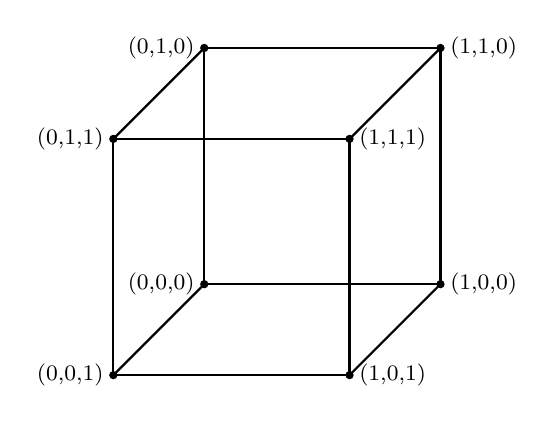
\begin{tikzpicture}[scale=3]
            % Define the coordinates for the cube
            \coordinate (A) at (0,0,0);
            \coordinate (B) at (1,0,0);
            \coordinate (C) at (1,1,0);
            \coordinate (D) at (0,1,0);
            \coordinate (E) at (0,0,1);
            \coordinate (F) at (1,0,1);
            \coordinate (G) at (1,1,1);
            \coordinate (H) at (0,1,1);
        
            % Draw the bottom face
            \draw[thick] (A) -- (B) -- (C) -- (D) -- cycle;
        
            % Draw the top face
            \draw[thick] (E) -- (F) -- (G) -- (H) -- cycle;
        
            % Draw the vertical edges
            \draw[thick] (A) -- (E);
            \draw[thick] (B) -- (F);
            \draw[thick] (C) -- (G);
            \draw[thick] (D) -- (H);

            % Add round points at each vertex
            \foreach \point in {(A), (B), (C), (D), (E), (F), (G), (H)}
                \fill \point circle (0.5pt);
        
            % Add labels with binary coordinates and adjusted positions
            \node[ left, font=\footnotesize] at (A) {(0,0,0)};
            \node[ right, font=\footnotesize] at (B) {(1,0,0)};
            \node[ right, font=\footnotesize] at (C) {(1,1,0)};
            \node[ left, font=\footnotesize] at (D) {(0,1,0)};
            \node[ left, font=\footnotesize] at (E) {(0,0,1)};
            \node[ right, font=\footnotesize] at (F) {(1,0,1)};
            \node[ right, font=\footnotesize] at (G) {(1,1,1)};
            \node[ left, font=\footnotesize] at (H) {(0,1,1)};
        
        \end{tikzpicture}
        \caption{3-dimensional hypercube.}
        \label{fig:hypercube}
    \end{figure}

    Given a (possibly empty) subset $T \subseteq [d]$ let $v_T \in \R^n$ be a vector, whose coordinates are indexed by $n=2^d$ vertices of the hypercube and defined by
    \begin{equation*}
        v_T(x) = (-1)^{\sum_{i \in T} x_i},
    \end{equation*}
    where $x_i$ is the $i$-th coordinate of the vertex $x\in\{0,1\}^d$.
    Also, let $S_T \subseteq V$ be the subset of vertices given by
    \begin{equation*}
        S_T = \brac{x \in V \colon v_T(x) = 1}.
    \end{equation*}
    \textit{[When $T = \emptyset$, we interpret the empty sum as zero, i.e. $\sum_{i \in \emptyset}x_i = 0$.]}
    
    \begin{enumerate}[(a)]
        \item Compute $h(S_{\brac{1}})$, the Cheeger's cut of the subset $S_{\brac{1}}$.

        \item Show that every vertex in $S_T$ has exactly $d-\abs{T}$ neighbours in $S_T$.
        
        \item Show that for any $T \subseteq [d]$, $v_T$ is an eigenvector of $\LL_G$ with eigenvalue $\frac{2\abs{T}}{d}$.
        
        \item Show that if $T' \subseteq [d]$ is distinct from $T$, then $v_T$ and $v_{T'}$ are orthogonal.

        \item Conclude that for any $0 \leq k \leq d$, the eigenspace corresponding to the eigenvalue $\frac{2k}{d}$ has dimension ${d \choose k}$.

        \item Compute $h_G$, the Cheeger’s constant of $G$.
    \end{enumerate}
\end{myexercise}

\begin{myexercise}[\level\level\level\sep Characterization of bipartite graphs]\label{prob:bipartite_graphs}
    Let $G = (V,E)$ be a graph.
    \begin{enumerate}[(a)]
        \item Prove that $G$ is bipartite if and only if there is no cycle of odd length.
        \item Prove that for any $k \geq 1$, $A^k$ is a matrix whose entry $(i, j)$ contains the number of paths of length $k$ between $i$ and $j$.
        \item Prove that $G$ is bipartite if and only if the spectrum of $A$ is symmetric, i.e. $\lambda_i(A) = - \lambda_{n+1-i}(A)$ for all $i \in [n]$.
        \item If in addition $G$ is connected and $d$-regular, prove that $G$ is bipartite if and only $\lambda_1(A) = - \lambda_n(A)$.
    \end{enumerate} 
\end{myexercise}
\begin{hint}
    (d): Try similar ideas as in the proof of the Gershgorin circle theorem, using $\lambda_n(A) = -d$.
\end{hint}




   





\begin{myexercise}
We will try various clustering methods on MNIST.  \\
(a) Implement your own version of Lloyd's k-means algorithm (do not use an existing k-means function; programming  it yourself will make you better aware of potential pitfalls or other aspects you need to pay attention to). Test it on MNIST. How well does k-means cluster the data? You need to come up with a performance metric to quantify what ``how well'' means (in case of MNIST we know the ground truth.). Also note that k-means may give you different results, based on different random initializations - how do you handle that?


\noindent
(b) Implement  spectral clustering and apply it to MNIST. There are parameters that you need to choose (a good value for $\sigma$, how may eigenvectors do you keep,...).
Recall that spectral clustering has a second step (the ``rounding step''), in which you use your k-means algorithm from (a) to cluster the spectrally-embedded data. As in (a), evaluate the performance of your clustering algorithm.
\end{myexercise}
